\documentclass{article}
\usepackage{amsmath}
\usepackage[utf8]{inputenc}
\usepackage[T1]{fontenc}
\usepackage[ngerman]{babel}
\usepackage[shortlabels]{enumitem}
\usepackage{amsfonts}
\usepackage[left=3cm,right=2cm,top=2.5cm,bottom=2cm]{geometry}
\usepackage{amssymb}
\usepackage{cancel}
\usepackage{karnaugh-map}
\usepackage{xcolor}

\title{Formale Grundlagen: Übung 3}
\author{Alexander Waldenmaier, Tutorin: Constanze Merkt}

\begin{document}
    \maketitle
    

    \subsection*{Aufgabe 3.1}
    Als Zwischenschritt definieren wir zunächst die Äquivalenz:
    \begin{align*}
        x \leftrightarrow y &= (x \rightarrow y) \wedge (y \rightarrow x)
    \end{align*}
    Damit lässt sich die Negation definieren:
    \begin{align*}
        \neg x &= x \leftrightarrow 0
    \end{align*}
    Wie aus dem Skript bekannt, ist $\{\neg, \wedge\}$ eine Basis. Demnach ist $\{\rightarrow, \wedge\}$ eine vollständige Basis.


    \subsection*{Aufgabe 3.2}
    \begin{enumerate}
        \item[a)] Überprüfung durch Wahrheitstabelle:\\\\
        \begin{tabular}{ccc|c|c}
            $A$ & $B$ & $C$ & $A \oplus (B \lor C)$ & $(A \oplus B) \lor (A \oplus C)$ \\
            \hline
            0 & 0 & 0 & 0 & 0 \\
            0 & 0 & 1 & 1 & 1 \\
            0 & 1 & 0 & 1 & 1 \\
            0 & 1 & 1 & 1 & 1 \\
            1 & 0 & 0 & 1 & 1 \\
            1 & 0 & 1 & 0 & 0 \\
            1 & 1 & 0 & 0 & 0 \\
            1 & 1 & 1 & 0 & 0
        \end{tabular}\\\\
        $\Rightarrow A \oplus (B \lor C) = (A \oplus B) \lor (A \oplus C)$
        \item[b)] Das Distributivgesetz ist hier nicht anwendbar, da es sich um eine Disjunktion und nicht eine Konjunktion handelt. Ein Gegenbeispiel ist $A=1, B=C=0$:
        \begin{align*}
            A \lor (B \oplus C) &\stackrel{!}{=} (A \lor B) \oplus (A \lor C) \\
            1 \lor (0 \oplus 0) &\stackrel{!}{=} (1 \lor 0) \oplus (1 \lor 0) \\
            1 \lor 0 &\stackrel{!}{=} 1 \oplus 1 \\
            1 &\neq 0 \\\\
            \Rightarrow A \lor (B \oplus C) &\neq (A \lor B) \oplus (A \lor C) 
        \end{align*}
    \end{enumerate}


    \subsection*{Aufgabe 3.3}
    % Im folgenden Karnaughdiagramm sind die Minterme von $F$ ihrer Reihenfolge nach nummeriert, nicht auftretende Konstellationen erhalten eine $0$. \\
    % \begin{karnaugh-map}[4][4][1][AC][DB]
    %     \manualterms{7,0,3,5,6,0,0,2,4,0,0,1,0,0,0,0}
    %     \implicant{3}{2}
    %     \implicantedge{0}{12}{2}{14}
    % \end{karnaugh-map}\\
    % $\Rightarrow F = \textcolor{green}{C} \lor \textcolor{red}{\bar{A}BD}$
    % \begin{minipage}[t]{0.16\textwidth}
    %     \begin{enumerate}
    %         \item $\bar{A}\bar{B}C\bar{D}$
    %         \item $\bar{A}\bar{B}CD$
    %         \item $\bar{A}B\bar{C}D$
    %         \item $A\bar{B}C\bar{D}$
    %         \item $\bar{A}BCD$
    %         \item $A\bar{B}CD$
    %         \item $ABCD$
    %     \end{enumerate}
    % \end{minipage}
    % \begin{minipage}[t]{0.03\textwidth}
    %     \vspace*{2cm}
    %     $\Rightarrow$
    % \end{minipage}
    % \begin{minipage}[t]{0.23\textwidth}
    %     \begin{enumerate}[a)]
    %         \item 1. und 2.: $\bar{A}\bar{B}C$
    %         \item 1. und 4.: $\bar{B}C\bar{D}$ 
    %         \item 2. und 5.: $\bar{A}CD$
    %         \item 2. und 6.: $\bar{B}CD$  
    %         \item 3. und 5.: $\bar{A}BD$
    %         \item 4. und 6.: $A\bar{B}C$
    %         \item 5. und 7.: $BCD$   
    %         \item 6. und 7.: $ACD$
    %     \end{enumerate}
    % \end{minipage}
    % \begin{minipage}[t]{0.03\textwidth}
    %     \vspace*{2cm}
    %     $\Rightarrow$
    % \end{minipage}
    % \begin{minipage}[t]{0.2\textwidth}
    %     \begin{enumerate}
    %         \item a) und f): $\bar{B}C$
    %         \item b) und d): $\bar{B}C$
    %         \item c) und d): $CD$
    %         \item c) und e): $\bar{A}D$
    %         \item c) und g): $CD$
    %         \item c) und h): $CD$
    %         \item 
    %     \end{enumerate}
    % \end{minipage}
    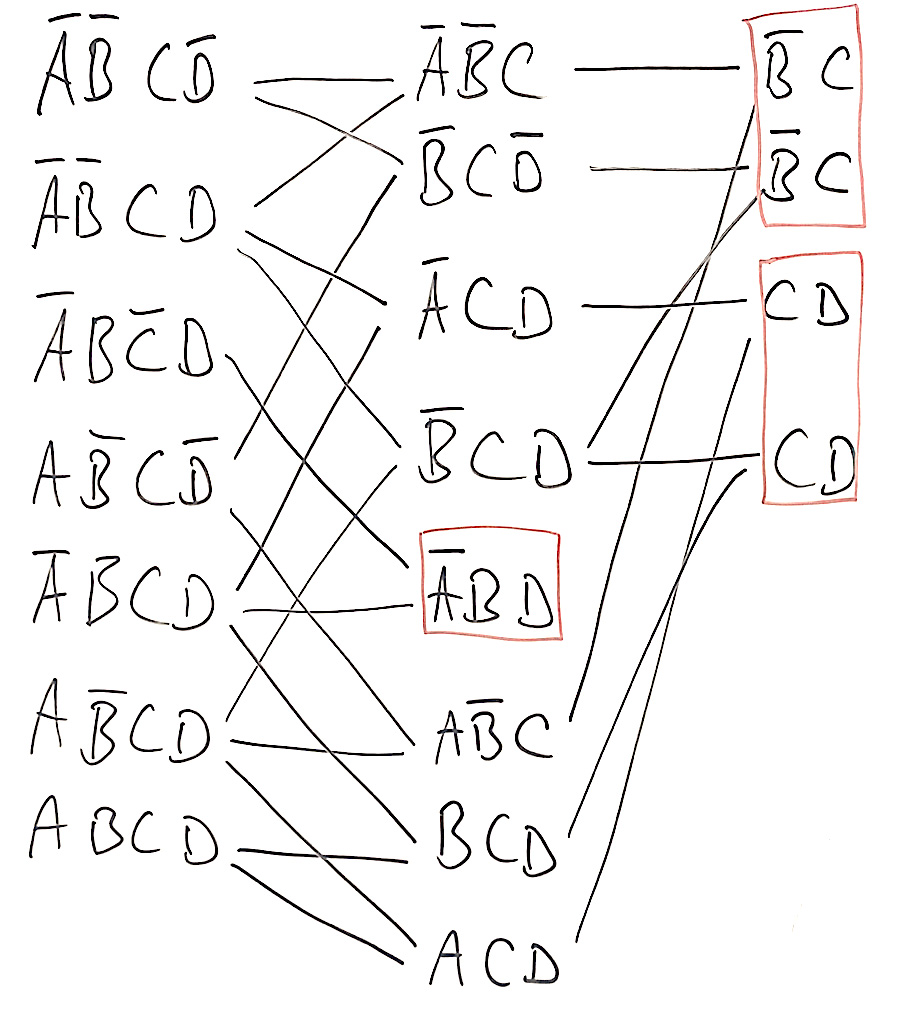
\includegraphics[width=0.4\textwidth]{Bild.jpg}\\\\
    \begin{tabular}{r|ccccccc}
        Minterm & 1 & 2 & 3 & 4 & 5 & 6 & 7 \\
        \hline
        $\bar{A}BD$ & &&+&&+&&\\
        $\bar{B}C$  & +&+&&+&&+&\\
        $CD$        & & +& & & +& + &+ 
    \end{tabular}\\\\\\
    $\Rightarrow F = \bar{A}BD \lor \bar{B}C \lor CD$

    \subsection*{Aufgabe 3.4}
    \begin{align*}
        F &= \neg(A \land \neg B) \land (\neg A \lor C) \land (\neg A \lor \neg(\neg B \land \neg C)) \\
        &= (1 \oplus (A \land (1 \oplus B))) \land \neg(A \land \neg C) \land \neg(A \lor (\neg B \land \neg C))\\
        &= (1 \oplus (A \oplus AB)) \land (1 \oplus (A \land (1 \oplus C))) \land \neg(A \lor \neg(B \lor C)) \\
        &= (1 \oplus A \oplus AB)  (1 \oplus (A \oplus AC))  (1 \oplus (A \land (1 \oplus (B \lor C)))) \\
        &= (1 \oplus A \oplus AB)  (1 \oplus A \oplus AC)  (1 \oplus (A \land ((1 \oplus B) \land (1 \oplus C)))) \\
        &= (1 \oplus A \oplus AC \oplus A \oplus A \oplus AC \oplus AB \oplus AB \oplus ABC)  (1 \oplus ((A \oplus AB)(1 \oplus C))) \\
        &= (1 \oplus A \oplus ABC)  (1 \oplus (A \oplus AC \oplus AB \oplus ABC)) \\
        &= (1 \oplus A \oplus ABC)  (1 \oplus A \oplus AB \oplus AC \oplus ABC) \\
        &= 1 \oplus A \oplus AB \oplus AC \oplus ABC \oplus A \oplus A \oplus AB \oplus AC \oplus ABC \oplus ABC \oplus ABC \oplus ABC \oplus ABC \oplus ABC  \\
        &= 1 \oplus A \oplus ABC \\\\
        \Rightarrow a &= (a_X)_{X \subseteq {1,...,n}} = (1, 1, 0, 0, 0, 0, 0, 1)
    \end{align*}


    \subsection*{Aufgabe 3.5}
    \begin{karnaugh-map}[4][4][1][AC][DB]
        \manualterms{0,0,1,1,0,0,0,1,1,1,0,0,1,1,1,1}
        \implicant{3}{7}
        \implicant{3}{2}
        \implicant{12}{9}
        \implicant{12}{14}
    \end{karnaugh-map}\\
    $\Rightarrow F = \textcolor{yellow}{\bar{A}D} \lor \textcolor{blue}{BD} \lor \textcolor{green}{A\bar{B}\bar{D}} \lor \textcolor{red}{AC\bar{D}}$ 
\end{document}